\section{Correlación}

La correlación es la premisa de la modelación predictiva, en el sentido de que es un factor con base en el cuál podemos predecir resultados.


Una buena correlación entre dos variables sugiere que existe una suerte de dependencia entre ambas:  Si una cambia, la otra también lo hará. 

Podemos decir que una buena correlación asegura una relación matemática entre dos variables y debido a esto, seremos capaces de predecir su comportamiento.


La relación puede ser de cualquier tipo.  Si $x$ y $y$ son dos variables correlacionadas, entonces podemos escribir:
\begin{align}
	Y=f(X)
\end{align}

\subsection{Ejemplos de correlación}
\begin{itemize}
	\item Correlación lineal
	\begin{align}
		y = ax+b
	\end{align}
	\item Correlación exponencial
	\begin{align}
		y = be^{ax}
	\end{align}
\end{itemize}


\subsection{Definición de correlación} Si $X,Y$ son dos variables aleatorias discretas, que pueden tomar valores $\set{x_{0},x_{1},...}$ y $\set{y_{0},y_{1},...}$, con promedios $\bar{x}, \bar{y}$  respectivamente, su correlación se define como
\begin{align}
	\corr(X,Y) = \dfrac{\sum_{x_{i},y_{j}}
		\left( \left( x_{i}-\bar{x} \right)\left( y_{j}-\bar{y} \right) \right)}
	{\sqrt{\sum_{x_{i},y_{j}}
			\left( x_{i}-\bar{x} \right)^{2}\sum_{x_{i},y_{j}}
			\left( y_{i}-\bar{y} \right)^{2}}}
\end{align}



\subsection{Propiedades de la correlación}
\begin{itemize}
	\item El valor del coeficiente de correlación está entre $-1$ y $1$, es decir $-1\leq  \corr(X,Y)  \leq 1.$ 
	\item Una correlación positiva significa una relación directa entre las dos variables. 
	\item Una correlación negativa significa una relación inversa entre las dos variables. 
	\item Entre mayor sea la magnitud del coeficiente, más fuerte será la relación entre variables.
\end{itemize}


\subsection{¡Advertencia!}
Aunque una correlación fuerte sugiere algún tipo de relación que puede ser utilizada para la predicción del comportamiento de una variable respecto de otra, \emph{esto no implica que dicha relación sea el único factor que explique dicho comportamiento.}


\begin{observacion}
	\emph{¡Correlación no implica causalidad!}
\end{observacion}



Por ejemplo, existe una correlación positiva muy fuerte entre el número de palabras que conoce un ser humano y el número de calzado que utiliza...  Pero esto esto se explica porque a medida que el ser humano crece, necesita zapatos más grandes y aprende palabras nuevas. 

\emph{¡No quiere decir que si utilizas un número más grande serás más culto!}


Tratemos de entender mejor este concepto mirando una base de datos y tratando de encontrar una correlación entre sus variables.  La base de datos que estaremos observando es una muy popular sobre los costos varios incurridos en \emph{publicidad por diferentes medios} y \emph{ventas de un producto en particular.}


Posteriormente, utilizaremos el método conocido como \emph{regresión lineal} para explorar estos mismo datos.

Por ahora, importemos esta base de datos y calculemos los coeficientes de correlación:

[,]{\texttt{advertising.py}}
\begin{lstlisting}[language=Python]
	#!/usr/bin/env python3
	# -*- coding: utf-8 -*-
	
	import pandas as pd
	
	advert = pd.read_csv("./dataBases/Advertising.csv")
	print(advert.head())
	
	import numpy as np
	
	advert["dX*dY"] = ( advert["TV"] -
	np.mean(advert["TV"])) * ( advert["Sales"]
	np.mean(advert["Sales"]))
	advert["dX**2"] = ( advert["TV"] -
	np.mean(advert["TV"])) ** 2
	advert["dY**2"] = ( advert["Sales"] -
	np.mean(advert["Sales"])) ** 2
	
	sxy = advert.sum()["dX*dY"]
	sxx = advert.sum()["dX**2"]
	syy = advert.sum()["dY**2"]
	
	r = sxy/np.sqrt(sxx*syy)
\end{lstlisting}


[,]{Salida de la pantalla}
\begin{lstlisting}[language=Python]
	TV  Radio  Newspaper  Sales
	0  230.1   37.8       69.2   22.1
	1   44.5   39.3       45.1   10.4
	2   17.2   45.9       69.3    9.3
	3  151.5   41.3       58.5   18.5
	4  180.8   10.8       58.4   12.9
\end{lstlisting}



[,]{\texttt{advertising2.py}}
\begin{lstlisting}[language=Python]
	#!/usr/bin/env python3
	# -*- coding: utf-8 -*-
	
	import pandas as pd
	
	advert = pd.read_csv("./dataBases/Advertising.csv")
	print(advert.head())
	
	import numpy as np
	
	def rCoef(df, var1, var2):
	df["dX*dY"] = (df[var1]-np.mean(df[var1]))*(df[var2]-np.mean(df[var2]))
	df["dX**2"] = (df[var1]-np.mean(df[var1]))**2
	df["dY**2"] = (df[var2]-np.mean(df[var2]))**2
	sxy = df.sum()["dX*dY"]
	sxx = df.sum()["dX**2"]
	syy = df.sum()["dY**2"]
	r = sxy/np.sqrt(sxx*syy)
	return r
	
	tvVsSales = rCoef(advert, "TV", "Sales")
	## 0.782224424862
	radioVsSales = rCoef(advert, "Radio", "Sales")
	## 0.576222574571
\end{lstlisting}




\begin{figure}
	\centering
	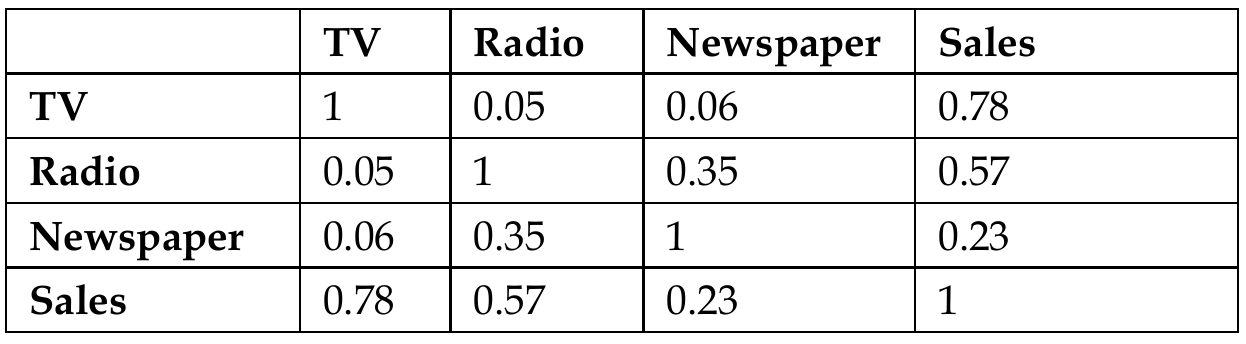
\includegraphics[width=10cm,keepaspectratio=true]{./images/correlationMatrix.png}
	% correlationMatrix.png: 0x0 pixel, 300dpi, 0.00x0.00 cm, bb=
	\caption{Matriz de correlación}
	\label{correlationMatrix}
\end{figure}



Veamos la naturaleza de esta correlación graficando las variables \texttt{TV}, \texttt{Radio} y \texttt{Newspaper} vs \texttt{Sales} del \textit{data frame} \texttt{advert}.

[,]{tvVsSales.py}
\begin{lstlisting}[language=Python]
	#!/usr/bin/env python3
	# -*- coding: utf-8 -*-
	
	import pandas as pd
	advert = pd.read_csv("./dataBases/Advertising.csv")
	
	import matplotlib.pyplot as plt
	
	plt.plot(advert['TV'],advert['Sales'],'ro')
	plt.title('TV vs Sales')
	plt.show()
	
	plt.plot(advert['Radio'],advert['Sales'],'ro')
	plt.title('Radio vs Sales')
	plt.show()
	
	plt.plot(advert['Newspaper'],advert['Sales'],'ro')
	plt.title('Newspaper vs Sales')
	plt.show()
\end{lstlisting}


\begin{center}
	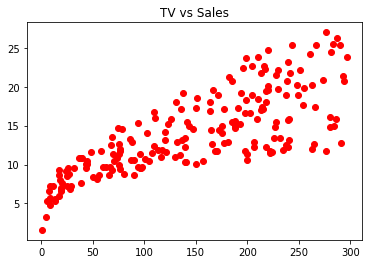
\includegraphics[width=10cm,keepaspectratio=true]{./images/tvVsSales.png}
	% tvVsSales.png: 0x0 pixel, 300dpi, 0.00x0.00 cm, bb=
\end{center}


\begin{center}
	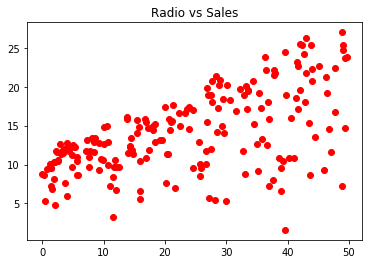
\includegraphics[width=10cm,keepaspectratio=true]{./images/radioVsSales.png}
	% tvVsSales.png: 0x0 pixel, 300dpi, 0.00x0.00 cm, bb=
\end{center}


\begin{center}
	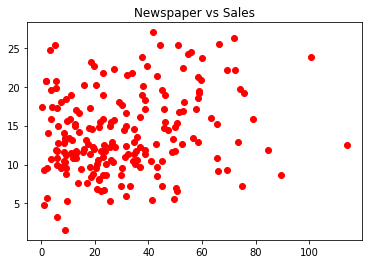
\includegraphics[width=10cm,keepaspectratio=true]{./images/newsVsSales.png}
	% tvVsSales.png: 0x0 pixel, 300dpi, 0.00x0.00 cm, bb=
\end{center}

